\documentclass[11pt]{article}
\usepackage[review]{acl}

% Math
\usepackage{amsmath,amssymb,amsfonts}

% Tables and figures
\usepackage{booktabs}
\usepackage{graphicx}
\usepackage{float}
\usepackage{multirow}
\usepackage{caption}
\usepackage{subcaption}

% References
\usepackage[numbers,sort&compress]{natbib}
\bibliographystyle{plainnat}

% Hyperlinks
\usepackage[colorlinks=true,citecolor=blue,linkcolor=blue,urlcolor=blue]{hyperref}

% Microtype
\usepackage{microtype}

% ============================================================
\title{LIF Gating Induces Selective Stabilization and \\
Depth-Dependent Organization Across Modalities}

\author{
  Kanako Yasukawa\thanks{Corresponding author.} \\
  Arizona State University (Online)\\
}

% ============================================================
\begin{document}
\maketitle

% ============================================================
\begin{abstract}
We introduce Leaky Integrate-and-Fire (LIF) gating, a minimal biologically-inspired mechanism (24--144 parameters) that acts as a selective stabilizer for Transformer language models. LIF produces two separable effects: (1)~variance reduction without mean loss penalty, and (2)~modality-dependent internal organization including depth hierarchy, head specialization, and emergent E/I balance. The effect is architecture-specific (Transformer but not CfC) and scale-dependent, with a U-shaped width dependence suggesting a critical threshold near 256d. At base scale ($N{=}8$), LIF leaves mean performance unchanged while reducing cross-seed variance by $1.2\times$. These patterns show structural parallels to biological neural organization, including inhibitory variability quenching and E/I-dependent critical periods.
\end{abstract}

% ============================================================
\section{Introduction}

Biological neural circuits exhibit progressive specialization, critical periods, and precise excitatory-inhibitory (E/I) balance, all emerging from simple local mechanisms. These principles are \emph{modality-independent}: the same GABAergic motifs produce different but analogous laminar organizations across sensory cortices \cite{douglas2004neuronal}. Artificial neural networks typically lack such self-organized structure.

We ask: \emph{can a minimal biologically-inspired gate induce biological-like organization in artificial networks across modalities?}

We introduce Ember, which augments standard architectures with Leaky Integrate-and-Fire (LIF) gates, the simplest model of neural spiking. Applied post-softmax in Transformers and post-hidden-state in CfC networks \cite{hasani2022closed}, the LIF gate adds only 24--144 parameters while producing organizational effects exceeding its parametric footprint. We evaluate on character-level text (Shakespeare) across multiple Transformer scales and a CfC baseline, and 35-class audio keyword spotting (Speech Commands v2 \cite{warden2018speech}).

Our key contributions:
\begin{enumerate}
    \item \textbf{Cross-modal regularization}: LIF acts as a stabilizer without loss penalty on text ($N{=}8$: $+0.01\%$, $p = 0.972$; variance $1.2\times$ reduction) and prevents catastrophic seed-dependent failures on audio (\S\ref{sec:text-results}--\ref{sec:seed1337}).
    \item \textbf{Spontaneous E/I balance}: Combining LIF with inhibitory mechanisms achieves $-0.45\%$ ($N{=}7$, $d{=}-0.58$) with seed-invariant critical periods (\S\ref{sec:ei-balance}--\ref{sec:critical-period}).
    \item \textbf{Architecture selectivity}: LIF regularizes Transformers (scale-dependent) but not text CfC, effective where content-dependent competition (softmax) occurs but not where sequential integration (ODE) dominates (\S\ref{sec:cross-arch}).
    \item \textbf{Width U-curve}: Critical threshold between 256d--320d (\S\ref{sec:width}).
    \item \textbf{In silico neuroanatomy}: LIF-gated networks provide a controlled experimental system where biological motifs can be inserted, removed, or replaced (e.g., SigmoidGate control), enabling causal experiments impossible in living tissue (\S\ref{sec:controls},~\S\ref{sec:neuroanatomy}).
\end{enumerate}


% ============================================================
\section{Method: LIF Gate Formulation}
\label{sec:method}

\subsection{Core Mechanism}

The LIF gate applies a threshold-based filter to neural activations. For input activation $x$:
\begin{equation}
    \text{fire\_mask} = \sigma(k \cdot (|x| - \theta))
    \label{eq:fire}
\end{equation}
\begin{equation}
    \text{smolder\_mask} = 1 - \text{fire\_mask}
    \label{eq:smolder}
\end{equation}
\begin{equation}
    y = x \odot (\text{fire\_mask} + \lambda \cdot \text{smolder\_mask})
    \label{eq:gate}
\end{equation}
\begin{equation}
    y = y \times \frac{\|x\|}{\|y\| + \varepsilon} \quad \text{(norm preservation, } \varepsilon = 10^{-8}\text{)}
    \label{eq:norm}
\end{equation}
where $\sigma$ is the sigmoid function, $\theta$ is the learnable threshold (initialized near 0 for identity behavior at startup), $k$ is the learnable steepness, and $\lambda$ is the learnable leak controlling sub-threshold transmission. The smolder mask (Eq.~\ref{eq:smolder}) prevents dead neurons by maintaining residual signal flow for sub-threshold activations, and norm preservation (Eq.~\ref{eq:norm}) rescales the output to match the input norm, ensuring that downstream LayerNorm statistics are not disrupted. This means LIF's effect is purely directional: it redistributes attention weight across heads without changing the overall magnitude of the representation.

\textbf{Gate position.} In Transformer Ember, the LIF gate is applied after attention probabilities are computed and before the attention output projection. In CfC variants (both text and audio), it is applied post-hidden-state, before the residual connection (Figure~\ref{fig:architecture}).

\begin{figure}[t]
\centering
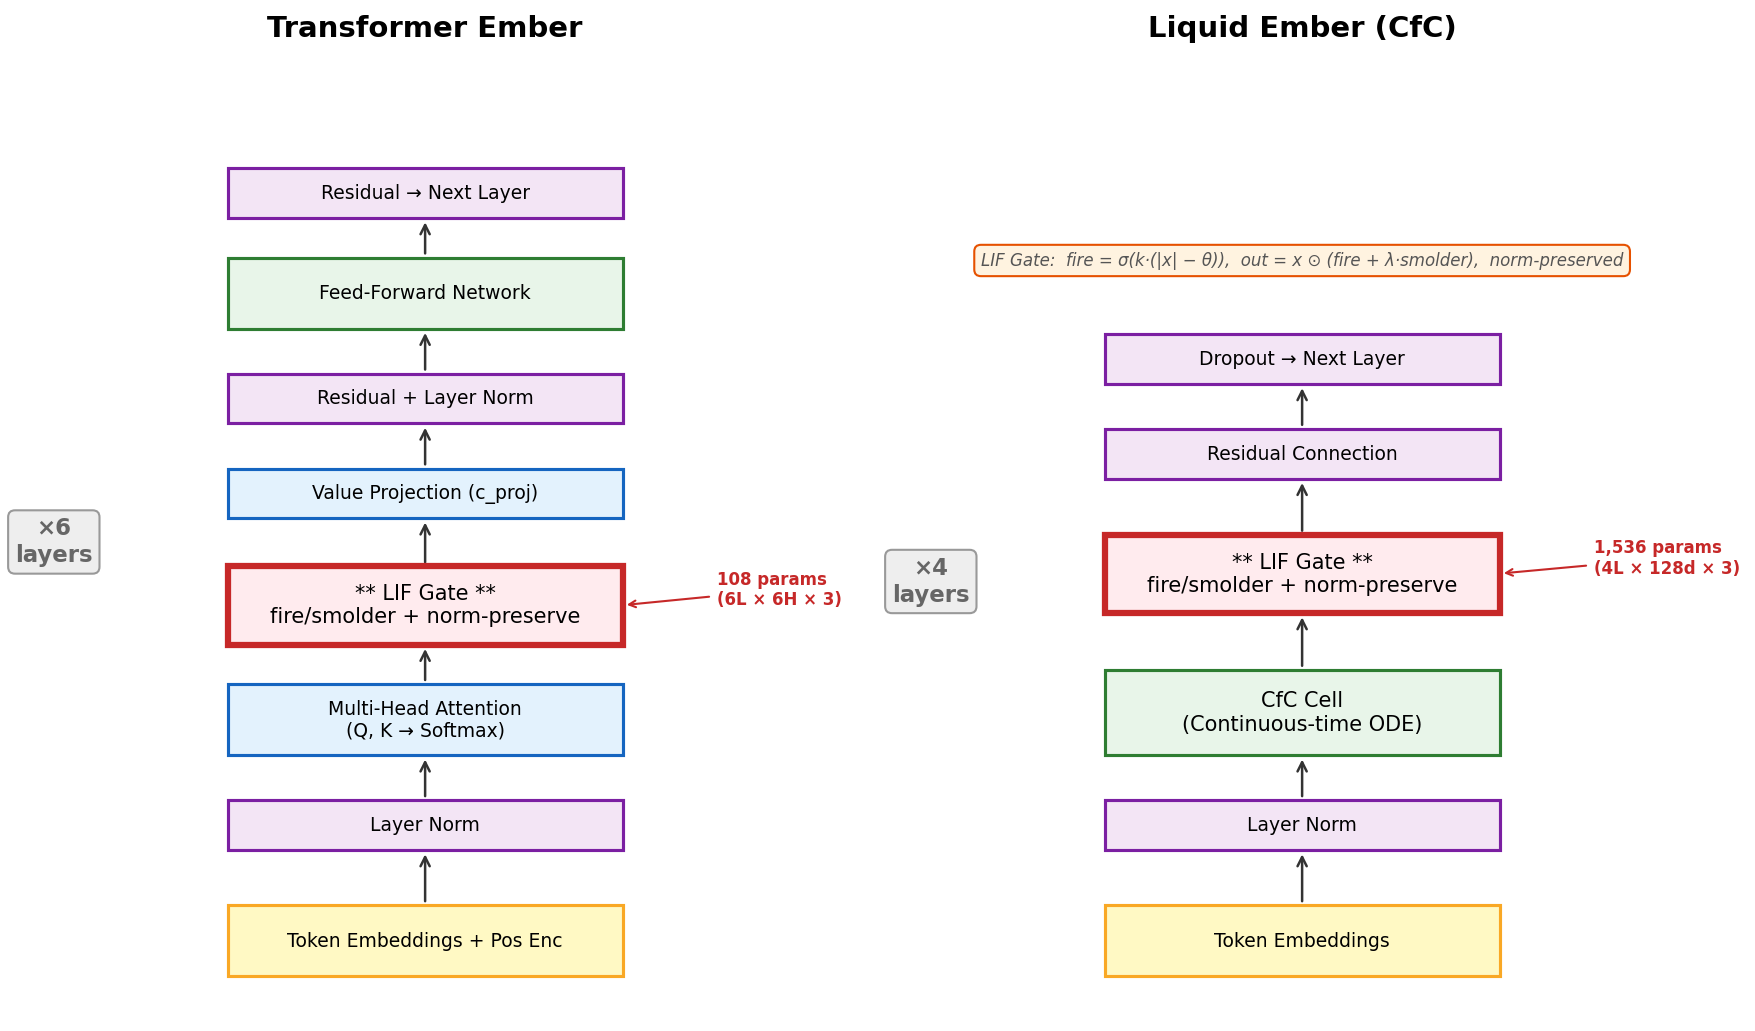
\includegraphics[width=0.85\textwidth]{figures/fig7_architecture.png}
\caption{\textbf{LIF gate position.} Transformer: post-softmax before $c\_proj$. CfC: post-hidden-state before residual. Eqs.~\ref{eq:fire}--\ref{eq:norm} define the gating with smolder mask and norm preservation.}
\label{fig:architecture}
\end{figure}

\textbf{v3.5 extensions (Transformer only).} We additionally test two inhibitory mechanisms:
\begin{itemize}
    \item \emph{Refractory period}: After firing, a gate unit enters a brief refractory state with elevated threshold, implementing local inhibition.
    \item \emph{Head-level persistence}: Gate state persists across tokens within a head, enabling temporal integration.
\end{itemize}

\subsection{Experimental Setup}

\textbf{Text.} Character-level Shakespeare (1.1M chars). Transformer base scale: 6L/6H/384d ($\sim$10.65M params), block\_size=256, 5,000 iterations, 8 seeds (42, 668, 1337, 2024, 314, 777, 1234, 99). Width sweep: 5 additional scales (128d--384d, varying depth/heads; Appendix Table~\ref{tab:cross-scale}), block\_size=128, 3,000 iterations, 3 seeds; extended 8-seed ablations at XS and Mid. E/I balance experiments: 3 seeds. CfC: 2--4 layers, 192--512 units. LIF adds 3 learnable parameters per head per layer (24--144 total in Transformers).

\textbf{Audio.} Speech Commands v2 \cite{warden2018speech}: 35-class, 105K utterances (1s, 16kHz). Mel spectrogram $\to$ 4-layer CfC (192 units) $\to$ classifier. $\sim$500K params + 1,536 LIF params. AdamW, 15 epochs, 6 seeds.


% ============================================================
\section{Results}

\subsection{Text: Transformer Full-Scale Ablation}
\label{sec:text-results}

\begin{table}[h]
\centering
\caption{Base-scale Transformer ablation (6L/6H/384d, $\sim$10.65M params, block\_size=256, 5000 iters). Standard vs LIF: $N{=}8$ seeds. E/I conditions: $N{=}7$ seeds (see Appendix Table~\ref{tab:ei-balance}).}
\label{tab:full-ablation}
\begin{tabular}{lcccc}
\toprule
\textbf{Condition} & \textbf{Val Loss} & \textbf{$\Delta$} & \textbf{Seeds Won} & \textbf{$N$} \\
\midrule
Standard (baseline) & $1.4820 \pm 0.0149$ & --- & --- & 8 \\
+ LIF gate only & $1.4822 \pm 0.0122$ & $+0.01\%$ & $4/8$ & 8 \\
\midrule
\multicolumn{5}{l}{\footnotesize E/I conditions below: $N{=}7$ seeds (seed 1337 excluded; no E/I run for this seed)} \\
Standard ($N{=}7$) & $1.4833 \pm 0.0168$ & --- & --- & 7 \\
+ Head-persist only & $1.4844 \pm 0.0213$ & $+0.07\%$ & $4/7$ & 7 \\
+ LIF + Refrac + Head & $1.4765 \pm 0.0140$ & $-0.45\%$ & $5/7$ & 7 \\
\bottomrule
\multicolumn{5}{l}{\footnotesize LIF-only ($N{=}8$): $t = 0.04$, $p = 0.972$, $d = 0.01$. Refrac+Head ($N{=}7$): $t = -1.53$, $p = 0.177$, $d = -0.58$.} \\
\end{tabular}
\end{table}

At base scale ($N{=}8$), LIF produces \textbf{no significant loss change} ($+0.01\%$, $p = 0.972$, Cohen's $d = 0.01$), with LIF winning exactly half the seeds (4/8). The initial 3-seed result ($-0.75\%$) was driven by seed 42 (a $-1.43\%$ outlier); the full 8-seed distribution is symmetric around zero. LIF reduces variance ($1.2\times$: std $0.0159 \to 0.0130$). When combined with inhibitory mechanisms (Refractory + Head-persistence), LIF achieves $-0.45\%$ ($N{=}7$, $p = 0.177$, $d = -0.58$), winning 5/7 seeds with variance reduction to $0.69\times$ (\S\ref{sec:ei-balance}). Head-persistence alone shows no effect ($+0.07\%$, $p = 0.822$).

\textbf{Scale dependence.} The LIF effect is strongly scale-dependent, forming a U-shaped curve across width (\S\ref{sec:width}). An 8-seed ablation at XS scale (2L/4H/128d) shows the strongest effect: paired $t$-test $t = 2.87$, $p = 0.024$ (uncorrected); Wilcoxon $W = 3.0$, $p = 0.039$; Cohen's $d = -1.02$; LIF wins 7/8 seeds. This $p$-value does not survive Bonferroni correction for five scale comparisons ($\alpha_{\text{adj}} = 0.01$); however, the large effect size ($d = -1.02$) and 7/8 seed consistency support a substantive effect that warrants targeted replication. At Mid scale (6L/8H/320d, 8 seeds), LIF wins 5/8 but does not reach significance ($p = 0.235$, Cohen's $d = -0.46$). At base scale, the effect vanishes entirely ($p = 0.972$). The width sweep reveals a U-shaped pattern (\S\ref{sec:width}): beneficial at 128d, harmful at 192--256d, and recovering at 320d+. The SigmoidGate control (\S\ref{sec:controls}) shows that at Wide scale, biological gate structure produces $10\times$ stronger regularization than smooth gating.

\subsection{Audio: CfC Classification}
\label{sec:audio-results}

On Speech Commands v2 (35-class keyword spotting, $N = 6$ seeds), CfC+LIF achieves $85.98\% \pm 0.37$ test accuracy vs.\ CfC-only $85.57\% \pm 0.77$ (mean $\Delta = +0.41\%$, $p = 0.395$ paired $t$-test, Cohen's $d = 0.42$). LIF wins 4/6 seeds. While not reaching significance at $N = 6$, the small-to-medium effect size ($d = 0.42$) and directional improvement (4/6 wins) suggest a trend that larger $N$ could clarify.

\textbf{Note on variance reduction estimates.} The original 3-seed subset (42, 668, 1337) showed $9.2\times$ validation variance reduction and $2.8\times$ test variance reduction. However, this was driven primarily by seed 1337's catastrophic baseline failure (\S\ref{sec:seed1337}), which inflated the baseline std. The full $N{=}6$ analysis shows test std ratio of $1.03\times$ (Base: 0.77, LIF: 0.37), indicating that LIF's audio benefit operates through \emph{floor-raising} (preventing worst-case outcomes) rather than uniform variance compression. Per-seed results are in Appendix Table~\ref{tab:audio-detail}.

\subsection{Illustrative Case: Seed 1337 Catastrophic Failure Prevention}
\label{sec:seed1337}

A single seed illustrates the underlying mechanism. In CfC-only with seed 1337, validation accuracy drops catastrophically at epoch 9 ($85.15\% \to 79.20\%$, $-5.95$ points), partially recovering to 86.51\% by epoch 14 (test: 84.59\%, worst of all runs). With CfC+LIF, epoch 9 validation is 86.53\% (improving, not collapsing); test: 86.19\%. LIF does not improve the ceiling; it \emph{raises the floor} (Appendix Figure~\ref{fig:seed1337}). This is a single-seed observation; generalizability depends on the aggregate statistics in Tables~\ref{tab:cross-modal} and \ref{tab:audio-detail}.

\subsection{Cross-Modal Comparison}
\label{sec:cross-modal}

\begin{table}[h]
\centering
\caption{Cross-modal summary: 2 backbones $\times$ 2 modalities $\times$ 2 tasks.}
\label{tab:cross-modal}
\begin{tabular}{lllcc}
\toprule
\textbf{Backbone} & \textbf{Modality} & \textbf{Task} & \textbf{Mean $\Delta$} & \textbf{Var Reduction} \\
\midrule
Transformer & Text & LM (loss) & $+0.01\%$ ($N{=}8$, $p{=}0.97$) & $1.2\times$ \\
CfC & Text & LM (loss) & $+0.14\%$ ($N{=}12$, $p{=}0.001$, $d{=}1.29$) & --- \\
CfC & Audio & Classification & $+0.41\%$ ($p{=}0.40$, $d{=}0.42$) & $1.03\times$ (test) \\
\bottomrule
\end{tabular}
\end{table}

LIF's effect is architecture-dependent. On Transformers, LIF is neutral at base scale ($+0.01\%$, $N{=}8$, $p{=}0.97$) while providing significant regularization at small scales (\S\ref{sec:width}). On CfC, LIF produces a significant degradation ($+0.14\%$, $N{=}12$, $p{=}0.001$, $d{=}1.29$; LIF wins 2/12 seeds), confirming architecture selectivity: LIF regularizes parallel attention (Transformer) but impairs sequential state update (CfC). Depth-entropy profiles are modality-dependent (Appendix Figure~\ref{fig:cross-modal-entropy}): Transformer text shows non-monotonic attention entropy with LIF amplifying the depth hierarchy (range ratio $1.27\times$); CfC text shows progressive neuron specialization from a verified zero-entropy baseline (all layers $p < 0.02$, Cohen's $d = 8$--$47$, $N{=}3$); CfC audio shows shallow-layer specialization (L0--L1 $p < 0.025$) with higher seed variance in deeper layers. CfC baseline operates in a complete firing regime (fire rate $= 1.0$, entropy $= 0$ across all seeds).

\subsection{Width Dependence}
\label{sec:width}

The LIF effect traces a \textbf{U-shaped curve} across 5 Transformer scales in the width sweep (Appendix Table~\ref{tab:cross-scale}; Figure~\ref{fig:ucurve}). Extended-seed analysis (8 seeds at XS and Mid, 7 seeds at Small, 3 seeds at Medium/Wide) reveals a gradual crossover across four regimes:

\begin{enumerate}
    \item \textbf{Small width (128d)}: LIF helps ($-0.068\%$, $p = 0.024$, $d = -1.02$, $N{=}8$).
    \item \textbf{Transitional width (192d)}: No detectable effect ($-0.023\%$, $p = 0.868$, $d = -0.071$, $N{=}7$).
    \item \textbf{All-needed width (256d)}: LIF hurts ($+0.355\%$, $p = 0.078$, $d = +1.95$, $N{=}3$).
    \item \textbf{Large width (320d+)}: LIF recovers ($-0.18\%$ at 320d, $-0.11\%$ at 384d).
\end{enumerate}

The critical crossover lies between 256d and 320d (Figure~\ref{fig:ucurve}). Per-head LIF threshold standard deviation decreases monotonically with width ($\sigma_\theta = 0.031$ at 128d to $0.016$ at 384d; Appendix Figure~\ref{fig:lif-pca-width}).

\begin{figure}[t]
\centering
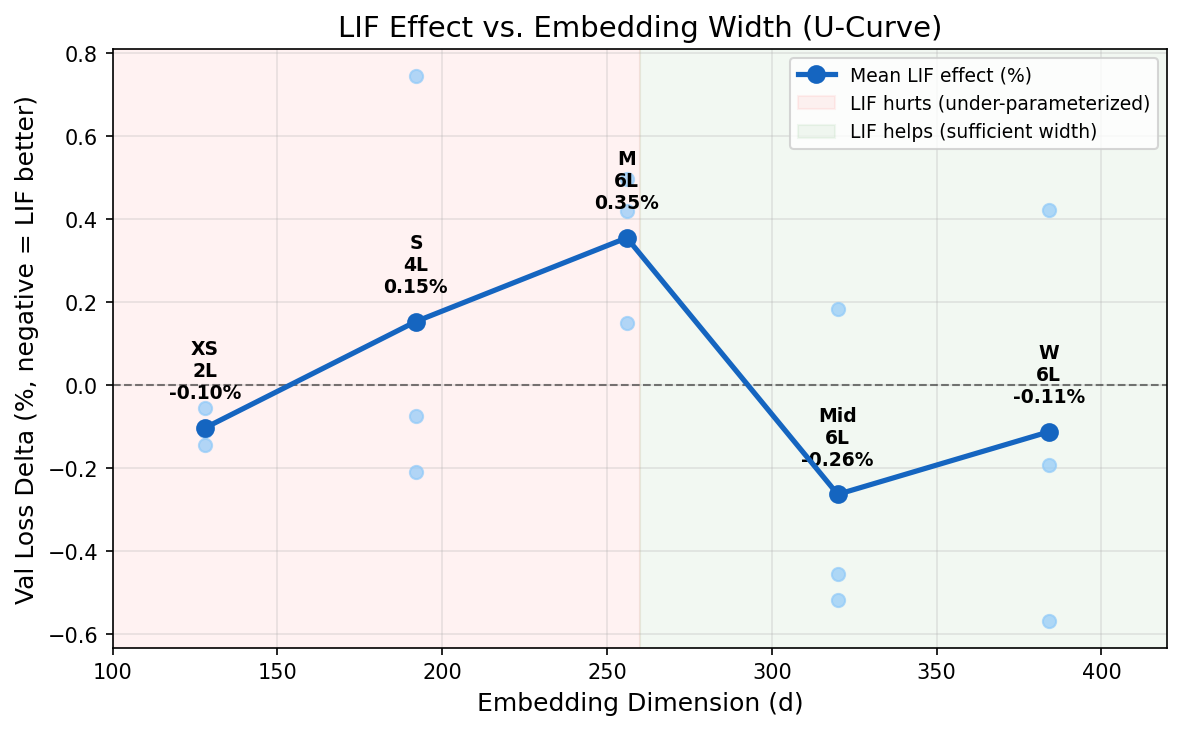
\includegraphics[width=0.7\textwidth]{figures/tiny_u_curve.png}
\caption{\textbf{U-shaped width dependence.} LIF delta (\%) across 5 scales. Critical crossover between 256d--320d separates harmful filtering (all dimensions needed) from beneficial regularization (redundancy exists). Extended 4-panel analysis in Appendix Figure~\ref{fig:ucurve-detail}.}
\label{fig:ucurve}
\end{figure}

\textbf{Width isolation.} Medium, Mid, and Wide share depth (6L) and head count (8H), differing only in \texttt{n\_embd}. At 256d, LIF hurts ($+0.35\%$, 0/3); at 320d, it helps ($-0.18\%$, $N{=}8$)---isolating width as the decisive variable. Cohen's $d$ also traces the U-curve: strong negative at XS ($d = -1.02$), positive through the middle ($d = +0.29$ to $+1.95$), returning negative at Mid and Wide ($d = -0.46$ to $-0.23$). Variance reduction tracks this curve: $40$--$86\%$ decrease where LIF helps, up to $68\%$ increase where it hurts. % Cortical minicolumn analogy moved to Discussion

\subsection{Cross-Architecture and Non-Biological Control}
\label{sec:cross-arch}
\label{sec:controls}

\textbf{Architecture selectivity.} LIF regularizes Transformers across text scales (significant at XS with $p = 0.024$; non-significant at base with $N{=}8$) while producing small but consistent degradation on CfC text ($+0.12\%$, $p = 0.0002$, $d = 0.35$, $N{=}9$; LIF wins 0/9; Appendix Table~\ref{tab:cross-arch}). LIF shows a non-significant positive trend on CfC audio ($+0.41\%$, $p = 0.395$, $d = 0.42$, $N{=}6$).

\textbf{SigmoidGate control.} To isolate biological structure from parameter count, we test a SigmoidGate with matched parameters at the identical position, without fire/smolder duality (Appendix Table~\ref{tab:controls}). At XS (128d), LIF $\equiv$ Sigmoid (pure parameter effect). At Medium (256d), both degrade equally (gate-generic). At Wide (384d), LIF is $10\times$ stronger ($-0.11\%$ vs $-0.01\%$). Above the width threshold, biological structure provides regularization that smooth gating cannot replicate.

% ============================================================
\section{Analysis}

\subsection{Critical Period and E/I Balance}
\label{sec:critical-period}
\label{sec:ei-balance}

At iteration $\sim$1600 ($\sim$53\% of training), LIF Transformers undergo a sharp transition: thresholds stabilize, head roles differentiate, and depth organization emerges. This timing is robust across seeds, paralleling biological critical periods \cite{hensch2005critical}: both are triggered by E/I balance maturation, endogenously timed, and produce selective circuit strengthening. Combining LIF (excitatory) with refractory+head-persistence (inhibitory) yields $-0.45\%$ ($N{=}7$, $p = 0.177$, Cohen's $d = -0.58$); head-persistence alone shows no improvement ($+0.07\%$, $p = 0.822$), confirming that E/I \emph{balance} is required (Appendix Table~\ref{tab:ei-balance}, Figure~\ref{fig:ei}). The medium effect size ($d = -0.58$) with enhanced variance reduction ($0.69\times$) suggests E/I balance strengthens LIF's stabilizer role. Post-critical-period, heads differentiate into pointer/gatherer/focuser roles with $\sim$25\% ``gatekeepers'' per layer (Appendix Figure~\ref{fig:head-params}), paralleling cortical inhibitory interneuron proportions (10--25\%; \cite{alizadeh2024ei}).


% ============================================================
\section{Discussion}

\subsection{Why Zero Loss Delta, Large Organizational Impact?}

At base scale ($N{=}8$), LIF produces no loss improvement whatsoever ($+0.01\%$, $p = 0.972$) while organizational changes persist (head specialization, E/I balance, depth hierarchy). This \textbf{honest null result} is itself informative: LIF is not an optimizer but a \emph{regularizer}. It likely acts through loss landscape modification: near-zero thresholds create smooth nonlinearities preventing sharp minima \cite{hochreiter1997flat,keskar2017large}, paralleling biological variability quenching \cite{churchland2010stimulus}. The primary value is \emph{stability and organization}, not peak performance, analogous to how biological gating mechanisms stabilize processing without enhancing raw computational power. This aligns with the contravariance principle \cite{cao2024contravariance}: when tasks are sufficiently difficult, systems that solve them converge toward functionally similar internal organization regardless of implementation details. LIF constrains this convergence without altering task performance.

\subsection{Neuroanatomical Correspondence}
\label{sec:neuroanatomy}

Table~\ref{tab:bio-comparison} provides quantitative comparison between LIF-emergent organization and biological cortical data.

\begin{table}[h]
\centering
\caption{Quantitative correspondence between LIF model and biological cortical data.}
\label{tab:bio-comparison}
\begin{tabular}{lccc}
\toprule
\textbf{Property} & \textbf{LIF Model} & \textbf{Biology} & \textbf{Source} \\
\midrule
Inhibitory ratio & $\sim$25\% & 10--25\% & \cite{alizadeh2024ei} \\
E/I ratio & 3:1 & 3:1--9:1 & \cite{alizadeh2024ei} \\
Layer-dep. E/I & Yes (entropy hier.) & Yes (L2/3: 5.25, L4: 7.34) & \cite{alizadeh2025layer} \\
Area-dep. E/I & Softmax-specific & Sensory: PV+, Assoc: SST+ & \cite{wang2020macroscale} \\
\bottomrule
\end{tabular}
\end{table}

The thalamus gates cortical (parallel) but not cerebellar (sequential) processing \cite{schmahmann1997cerebrocerebellar}. LIF mirrors this: effective on Transformer attention but not on CfC text. LIF appears \emph{softmax-specific}: CfC (ODE-based, no softmax) shows small but consistent degradation ($+0.12\%$, $N{=}9$, $p = 0.0002$, $d = 0.35$; LIF wins 0/9), consistent with the hypothesis that threshold gating is effective only where content-dependent competition (softmax) occurs. Per-head gatekeeper specialization ($\sim$25\%) falls within the biological range of inhibitory interneuron proportions (10--25\%; \cite{alizadeh2024ei}). The U-curve width dependence (Figure~\ref{fig:ucurve}) suggests that representational capacity, not volume, determines LIF effectiveness, consistent with avian brains achieving primate-level cognition through neuronal density \cite{olkowicz2016birds}. We use ``parallels'' deliberately: these are structural correspondences, not mechanistic equivalences.

\subsection{Limitations}

\textbf{Base-scale null result}: The $N{=}8$ ablation shows no significant loss improvement at base scale ($p = 0.972$). The initial 3-seed result ($-0.75\%$) did not replicate. \textbf{Statistical power}: XS 8-seed reaches nominal significance ($p = 0.024$, uncorrected; exploratory across 5 scales), but Mid ($p = 0.235$), Audio ($p = 0.395$), and Base ($p = 0.972$) do not. E/I balance ($N{=}7$) shows medium effect ($d = -0.58$, $p = 0.177$) but does not reach significance. \textbf{Tasks}: One text and one audio task; vision, multi-task, and continuous speech untested. \textbf{Controls}: SigmoidGate tested at 3 scales ($N{=}3$). \textbf{CfC}: Text result ($N{=}9$, $p = 0.0002$, $d = 0.35$, LIF wins 0/9) shows small but significant degradation, strengthening the softmax-specificity hypothesis; additional non-softmax backends remain desirable. \textbf{Seed 1337}: Single-seed case study. \textbf{Analogies}: We claim functional correspondence, not structural equivalence.


% ============================================================
\section{Related Work}

\textbf{Regularization.}
Dropout \cite{srivastava2014dropout}, stochastic depth \cite{huang2016stochastic}, and batch normalization \cite{ioffe2015batch} operate on individual neurons, layers, or activation statistics. SAM \cite{foret2021sharpnessaware} seeks flat minima at the optimizer level. LIF differs by gating at the \emph{attention head} level with \emph{persistent} threshold state across tokens. Critically, dropout reduces variance but does not induce head specialization; LIF does both.

\textbf{Sparse/gated attention and SNNs.}
Sparse Transformers \cite{child2019generating}, MoE \cite{fedus2022switch}, and Lottery Tickets \cite{frankle2019lottery} exploit the insight that not all capacity is needed at all times. Qwen \cite{yang2025qwen3} uses sigmoid gates ($884$K params) per head. LIF uses $8{,}000\times$ fewer parameters with learned thresholds rather than fixed patterns. Unlike full SNN approaches \cite{maass1997networks,zhou2023spikformer,bellec2018long}, we transplant a single biological motif into standard attention, preserving floating-point computation while inheriting threshold-based organizational properties.

\textbf{Neuroscience connections.}
Flat minima correlate with generalization \cite{hochreiter1997flat,keskar2017large}; LIF may achieve flatness through threshold-induced smoothing. Simpler feedforward architectures can better align with brain hierarchy than complex ones \cite{nonaka2021brain}, suggesting that minimal biological constraints may be more effective than detailed mimicry. Stimulus-onset variability quenching \cite{churchland2010stimulus}, a trial-to-trial phenomenon within individual neurons, provides a biological analog at a different level of analysis: LIF reduces cross-seed variance (between models with different initializations) whereas quenching reduces trial-to-trial variance (within a single system). E/I balance is required for robust selectivity \cite{mackwood2021ei,rubin2017balanced,douglas2004neuronal}; our $\sim$75/25\% head ratio emerges through training dynamics (whether from initialization drift or self-organization remains an open question). Critical periods are gated by E/I maturation \cite{hensch2005critical,bengio2009curriculum}; our threshold crossover at iteration $\sim$1600 parallels this developmental transition. Gan \& Isola \cite{gan2026neural} show that diverse task experts densely populate the neighborhood of pretrained weights; LIF gating can be understood as a biologically-grounded mechanism for selectively activating these pre-existing experts via E/I-controlled threshold dynamics.


% ============================================================
\section{Conclusion}

LIF gating (24--144 parameters) produces two separable effects: \textbf{selective stabilization}: variance reduction without loss penalty on text ($N{=}8$: $+0.01\%$, $p = 0.972$) and consistent floor-raising on audio; and \textbf{modality-dependent organization}: depth hierarchy, head specialization, and emergent E/I balance ($N{=}7$: $-0.45\%$, $d = -0.58$). LIF regularizes Transformers (significant at small scales, stabilizing at larger scales) but not CfC text, consistent with softmax-specific gating selectivity. The honest null result at base scale is itself a finding: LIF acts as a stabilizer, not an optimizer. E/I balance strengthens this role: inhibition alone has no effect, but combined with LIF gating, it produces medium-effect improvement with enhanced variance reduction. The brain may spike not to save power or improve accuracy, but to \emph{organize and stabilize} parallel computation---and artificial networks, given the minimal constraint of a threshold gate, arrive at functionally similar solutions.


% ============================================================
\section*{Acknowledgments}

Claude (Anthropic) was used for code implementation, experimental execution, data analysis, and drafting assistance. All scientific decisions, experimental design, interpretation of results, and final content were reviewed and approved by the human author.

% ============================================================
\clearpage
\appendix

\section*{Appendix A: Detailed Tables and Figures}

\begin{figure}[h]
\centering
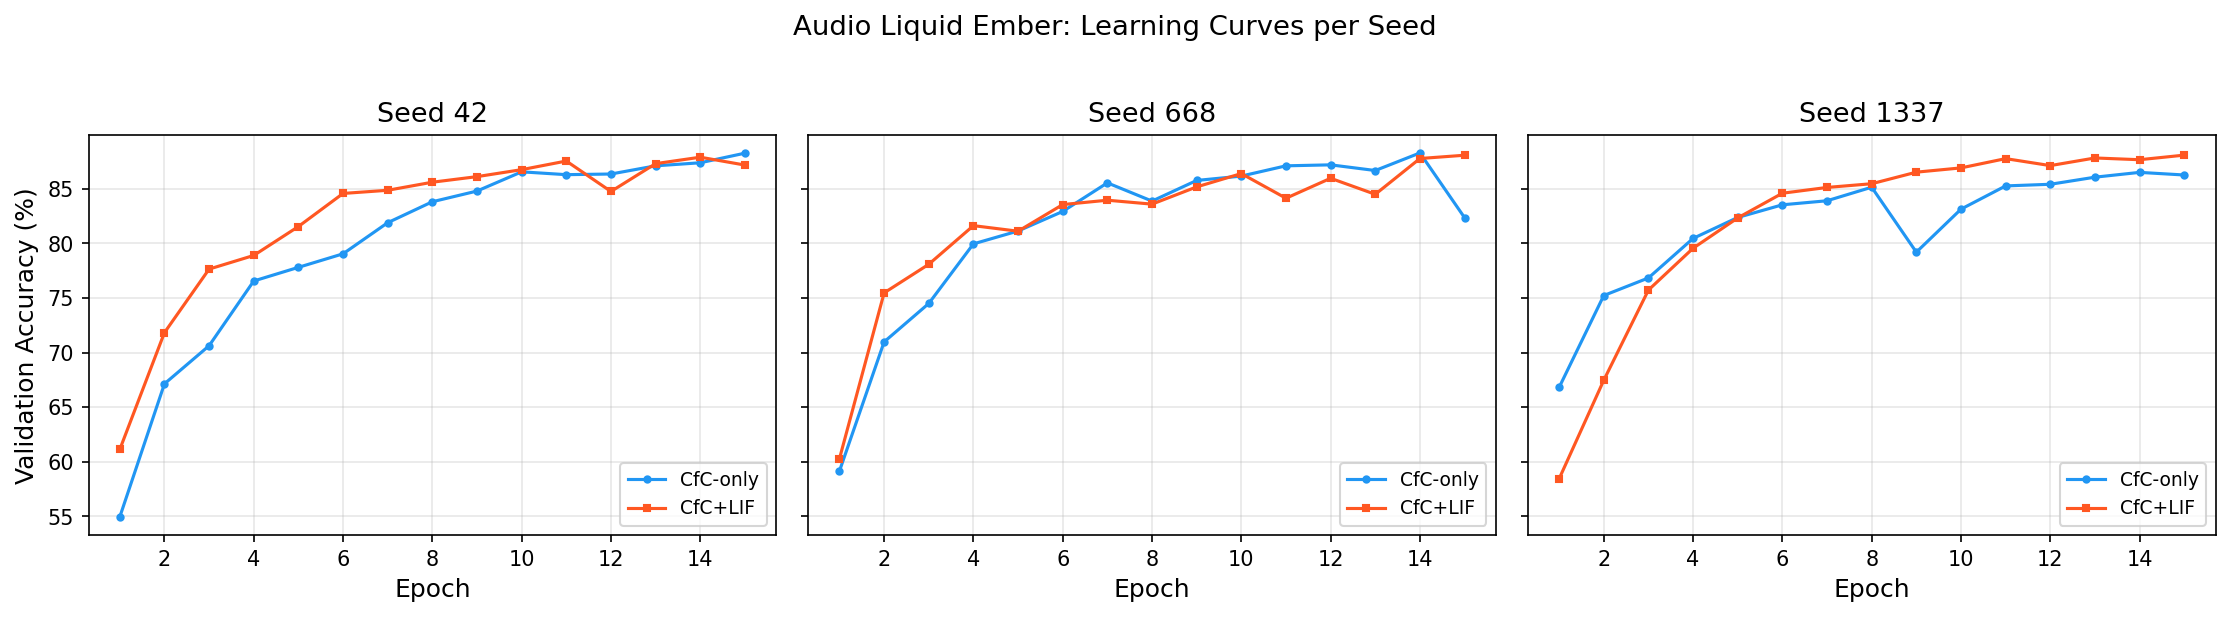
\includegraphics[width=0.75\textwidth]{figures/audio_fig2_learning_curves.png}
\caption{\textbf{Seed 1337 case study.} CfC-only shows catastrophic validation collapse at epoch 9 ($-5.95$ points), absent in CfC+LIF. This illustrates the mechanism underlying aggregate variance reduction.}
\label{fig:seed1337}
\end{figure}

\begin{table}[h]
\centering
\caption{v3.5 E/I balance results (6L/6H/384d, base scale, $N{=}7$). $\Delta$ relative to 7-seed Standard mean. Head-persist alone shows no improvement; only the combination with LIF gating produces consistent benefit, confirming E/I balance is required.}
\label{tab:ei-balance}
\begin{tabular}{lccccc}
\toprule
\textbf{Condition} & \textbf{Val Loss} & \textbf{$\Delta$} & \textbf{Wins} & \textbf{$p$} & \textbf{$d$} \\
\midrule
Standard ($N{=}7$) & $1.4833 \pm 0.0168$ & --- & --- & --- & --- \\
+ Head-persist only & $1.4844 \pm 0.0213$ & $+0.07\%$ & $4/7$ & $0.822$ & $0.09$ \\
+ \textbf{LIF + Refrac + Head} & $\mathbf{1.4765 \pm 0.0140}$ & $\mathbf{-0.45\%}$ & $\mathbf{5/7}$ & $0.177$ & $-0.58$ \\
\bottomrule
\multicolumn{6}{l}{\footnotesize Var ratio: HP $1.62\times$ (increased), RH $0.69\times$ (reduced). Paired $t$-tests.} \\
\end{tabular}
\end{table}

\begin{table}[h]
\centering
\caption{Width sweep: LIF effectiveness across 5 Transformer scales (block\_size=128, 3000 iters). $^\dagger$8-seed extended ablation; Small 7-seed extended ablation; Medium/Wide 3-seed. Base-scale result (6L/6H/384d) in Table~\ref{tab:full-ablation} uses different training setup.}
\label{tab:cross-scale}
\begin{tabular}{lccccccc}
\toprule
\textbf{Scale} & \textbf{Config} & \textbf{$N$} & \textbf{$\Delta$} & \textbf{$p$} & \textbf{$d$} & \textbf{Regime} \\
\midrule
XS$^\dagger$ & 2L/4H/128d & 8 & $-0.068\%$ & $0.024$ & $-1.02$ & Constrained \\
Small & 4L/4H/192d & 7 & $-0.023\%$ & $0.868$ & $-0.071$ & Neutral \\
Medium & 6L/8H/256d & 3 & $+0.355\%$ & $0.078$ & $+1.95$ & All-needed \\
Mid$^\dagger$ & 6L/8H/320d & 8 & $-0.178\%$ & $0.235$ & $-0.46$ & Redundant \\
Wide & 6L/8H/384d & 3 & $-0.113\%$ & $0.728$ & $-0.23$ & Redundant \\
\bottomrule
\end{tabular}
\end{table}

\begin{table}[h]
\centering
\caption{Audio classification per-seed results (Speech Commands v2, 35 classes, $N = 6$).}
\label{tab:audio-detail}
\begin{tabular}{llccl}
\toprule
\textbf{Condition} & \textbf{Seed} & \textbf{Test Acc (\%)} & \textbf{$\Delta$} & \textbf{Winner} \\
\midrule
CfC-only & 42 & 86.56 & & \\
CfC-only & 668 & 86.25 & & \\
CfC-only & 1337 & 84.59 & & \\
CfC-only & 2024 & 84.84 & & \\
CfC-only & 314 & 85.72 & & \\
CfC-only & 777 & 85.45 & & \\
\cmidrule{2-5}
& Mean $\pm$ std & $85.57 \pm 0.77$ & & \\
\midrule
CfC+LIF & 42 & 85.42 & $-1.14$ & Base \\
CfC+LIF & 668 & 85.80 & $-0.45$ & Base \\
CfC+LIF & 1337 & 86.19 & $+1.60$ & LIF \\
CfC+LIF & 2024 & 86.22 & $+1.38$ & LIF \\
CfC+LIF & 314 & 85.85 & $+0.13$ & LIF \\
CfC+LIF & 777 & 86.40 & $+0.95$ & LIF \\
\cmidrule{2-5}
& Mean $\pm$ std & $85.98 \pm 0.37$ & $+0.41$ & 4W/2L \\
\midrule
\multicolumn{5}{l}{Paired $t$-test: $t = 0.93$, $p = 0.395$; Cohen's $d = 0.42$} \\
\bottomrule
\end{tabular}
\end{table}

\begin{table}[h]
\centering
\caption{Cross-architecture comparison at matched scales. $^\dagger$8-seed; $^*$base scale (block\_size=256, 5000 iters); others 3-seed with block\_size=128, 3000 iters. Base row updated to $N{=}8$.}
\label{tab:cross-arch}
\begin{tabular}{llccc}
\toprule
\textbf{Architecture} & \textbf{Scale} & \textbf{Standard} & \textbf{+LIF} & \textbf{$\Delta$} \\
\midrule
Transformer$^\dagger$ & XS (128d) & 1.6167 & 1.6156 & $-0.068\%$ \\
Transformer$^\dagger$ & Mid (320d) & 1.4768 & 1.4741 & $-0.178\%$ \\
Transformer & Wide (384d) & 1.4862 & 1.4845 & $-0.12\%$ \\
Transformer$^{*\dagger}$ & Base (384d) & 1.4820 & 1.4822 & $+0.01\%$ \\
\midrule
CfC (text) & XS (128d) & 1.6375 & 1.6392 & $+0.10\%$ \\
CfC (text) & Wide (384d) & 1.4851 & 1.4852 & $+0.01\%$ \\
\bottomrule
\end{tabular}
\end{table}

\begin{table}[h]
\centering
\caption{Non-biological gate control: LIF vs Sigmoid at matched parameters (3 per head per layer).}
\label{tab:controls}
\begin{tabular}{llccc}
\toprule
\textbf{Scale} & \textbf{Gate} & \textbf{Val Loss} & \textbf{$\Delta$ vs Std} & \textbf{vs LIF} \\
\midrule
\multirow{3}{*}{XS (128d)} & Standard & $1.6171 \pm 0.0060$ & --- & --- \\
 & LIF & $1.6155 \pm 0.0058$ & $-0.10\%$ & --- \\
 & Sigmoid & $1.6155 \pm 0.0058$ & $-0.10\%$ & $\equiv$ LIF \\
\midrule
\multirow{3}{*}{Medium (256d)} & Standard & $1.4736 \pm 0.0022$ & --- & --- \\
 & LIF & $1.4788 \pm 0.0037$ & $+0.35\%$ & --- \\
 & Sigmoid & $1.4796 \pm 0.0020$ & $+0.41\%$ & $\approx$ LIF \\
\midrule
\multirow{3}{*}{Wide (384d)} & Standard & $1.4862 \pm 0.0113$ & --- & --- \\
 & LIF & $1.4845 \pm 0.0067$ & $-0.11\%$ & --- \\
 & Sigmoid & $1.4860 \pm 0.0061$ & $-0.01\%$ & $10\times$ weaker \\
\bottomrule
\end{tabular}
\end{table}

\begin{figure}[h]
\centering
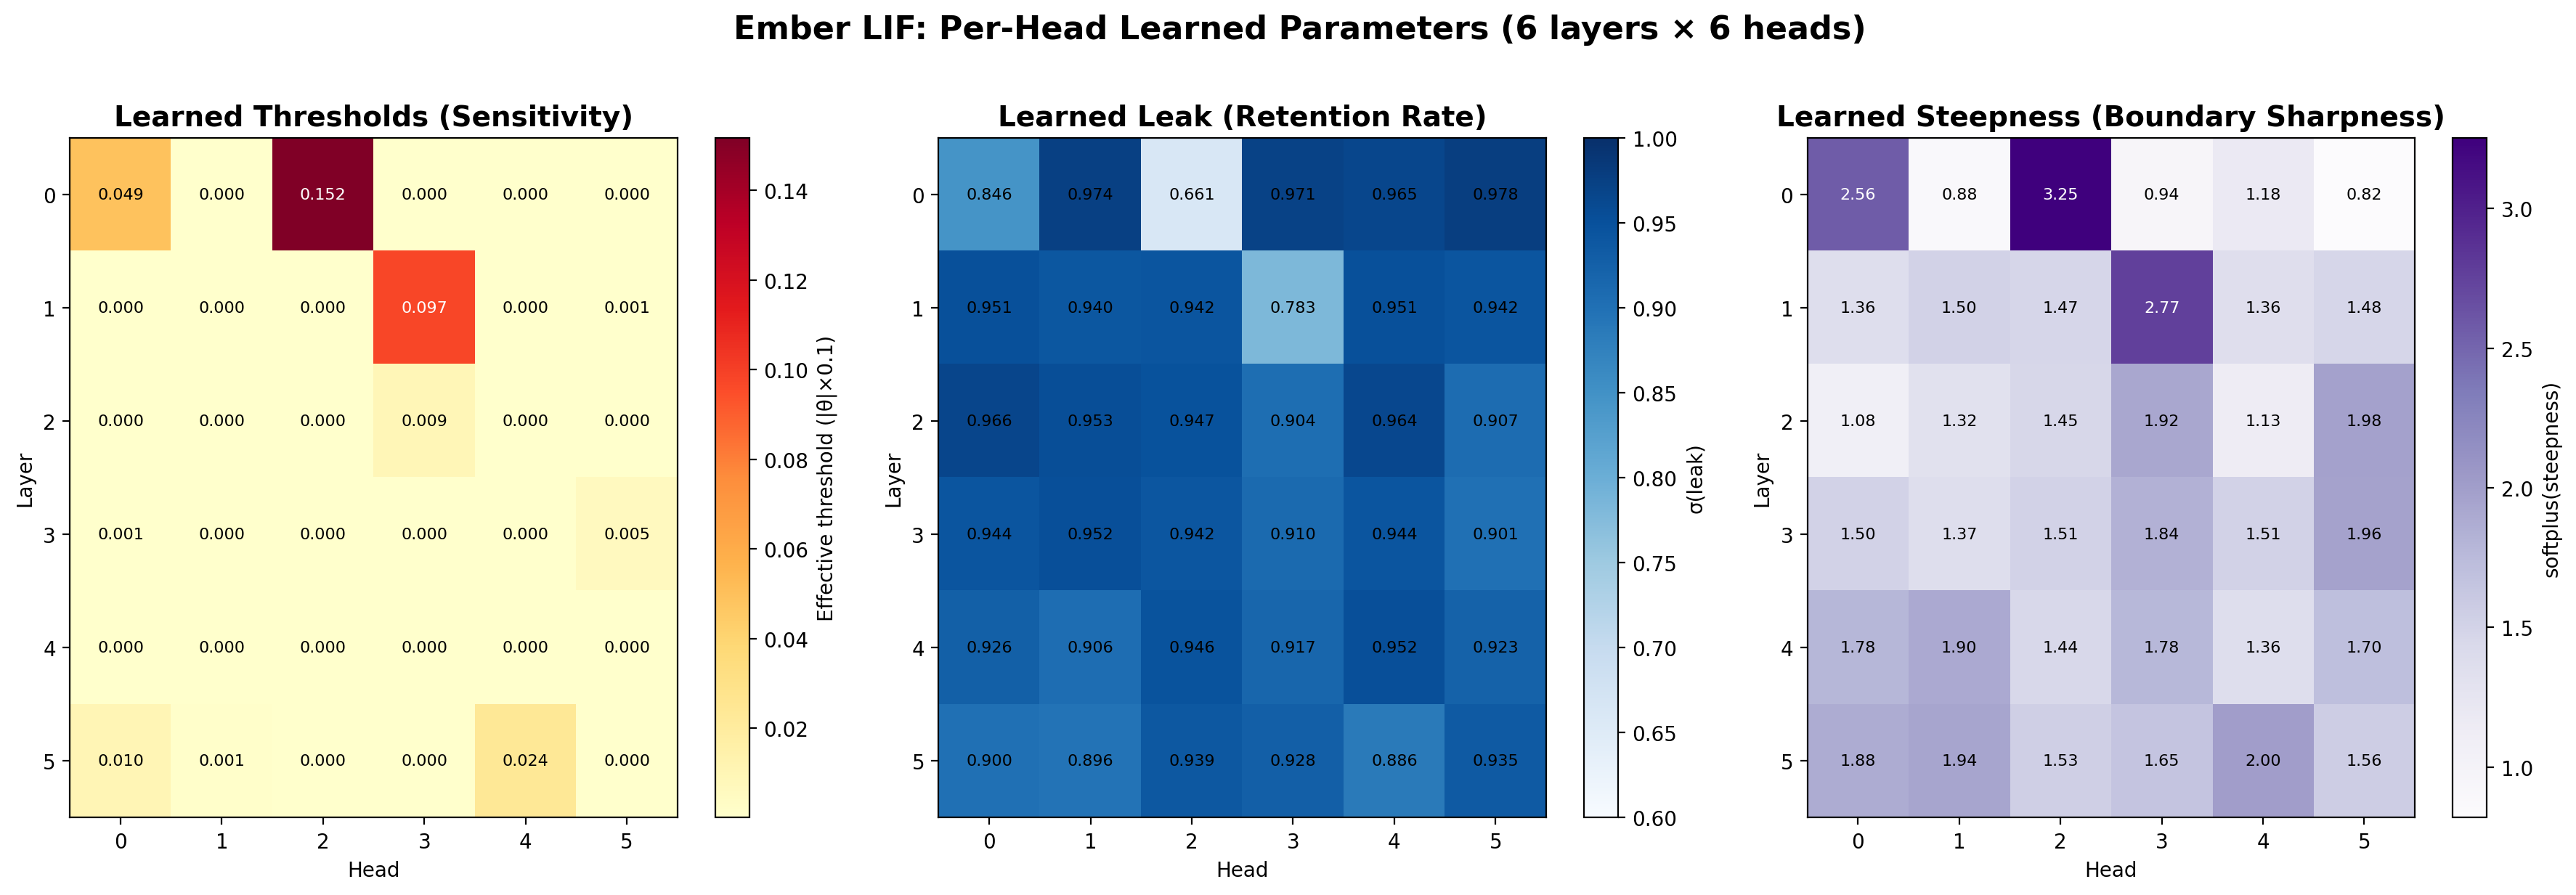
\includegraphics[width=0.85\textwidth]{figures/lif_head_parameters.png}
\caption{\textbf{Per-head learned LIF parameters (wide scale).} Heatmaps of threshold, leak, and steepness across layers and heads. One head per layer consistently emerges as a high-threshold outlier, with coordinated extremity across all three parameters suggesting functional gatekeeper specialization ($\sim$25\% per layer).}
\label{fig:head-params}
\end{figure}

\begin{figure}[h]
\centering
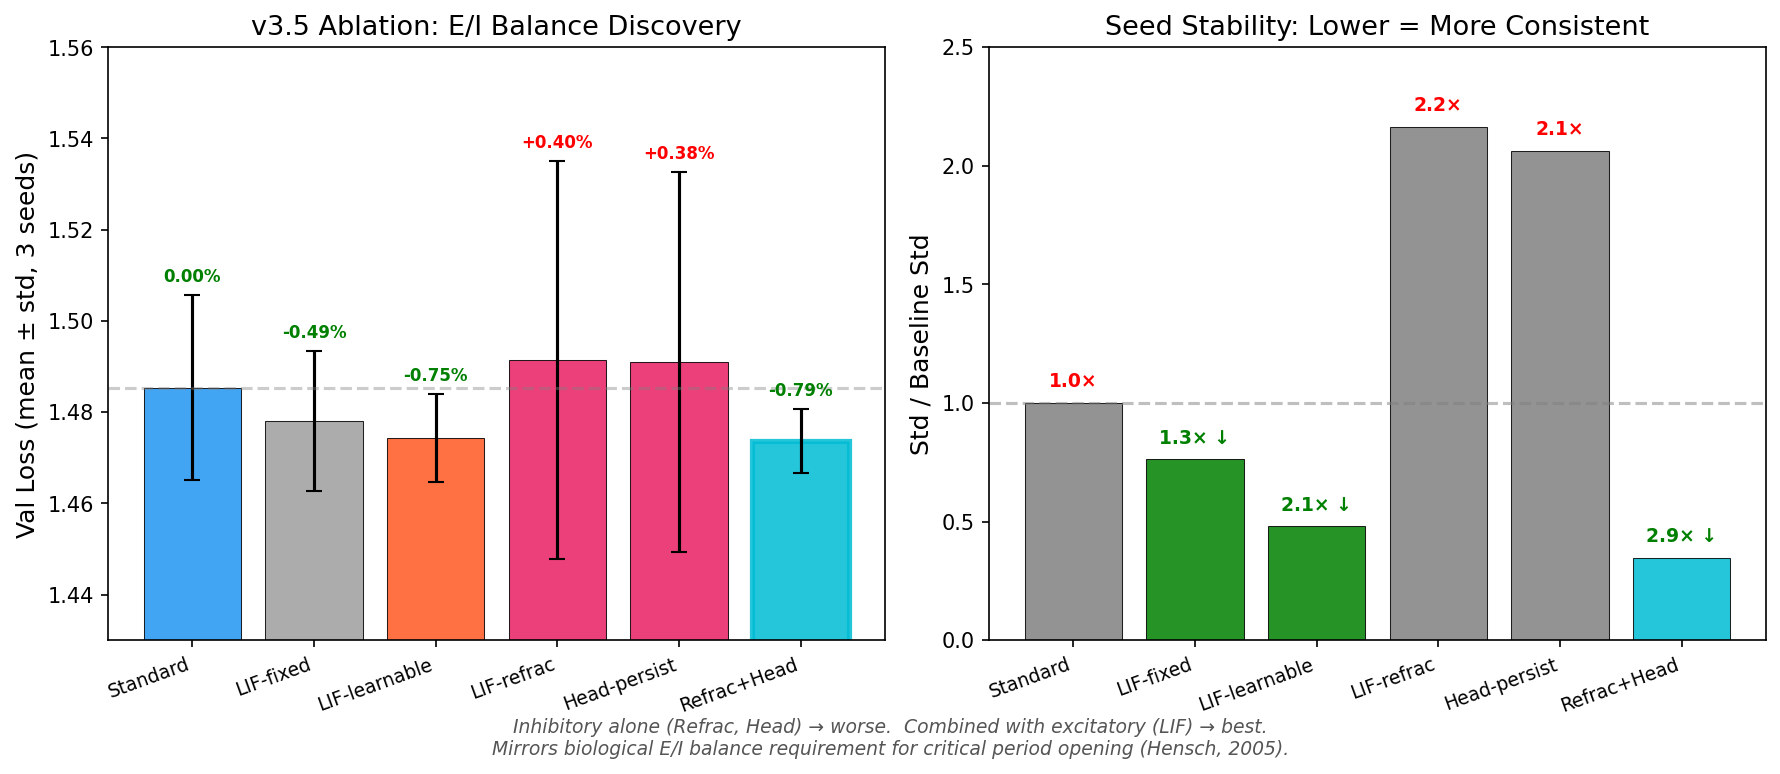
\includegraphics[width=0.85\textwidth]{figures/fig6_ei_balance.png}
\caption{\textbf{v3.5 E/I balance ($N{=}7$).} Head-persistence alone has no effect ($+0.07\%$, $p = 0.822$); combined with LIF gating, it achieves $-0.45\%$ ($p = 0.177$, $d = -0.58$) with enhanced variance reduction ($0.69\times$). This parallels the biological requirement for both E and I components in critical period opening \cite{hensch2005critical}.}
\label{fig:ei}
\end{figure}

\begin{figure}[h]
\centering

\includegraphics[width=\textwidth]{figures/fig_cross_modal_entropy.png}
\caption{\textbf{Cross-modal depth-entropy profiles (verified from checkpoints).} Left: Transformer text attention entropy shows non-monotonic profile; LIF amplifies the depth hierarchy (range $1.27\times$). Center: CfC text neuron firing entropy (N=3 seeds, error bars = cross-seed std); base entropy is exactly zero (fire rate $= 1.0$), LIF creates progressive differentiation (all layers $p < 0.02$). Right: CfC audio (N=6 seeds); LIF specialization is concentrated in shallow layers (L0--L1 $p < 0.025$) with high seed variance in deeper layers. Common feature: LIF induces depth-dependent organization absent in baselines (\S\ref{sec:cross-modal}).}
\label{fig:cross-modal-entropy}
\end{figure}

\begin{figure}[h]
\centering
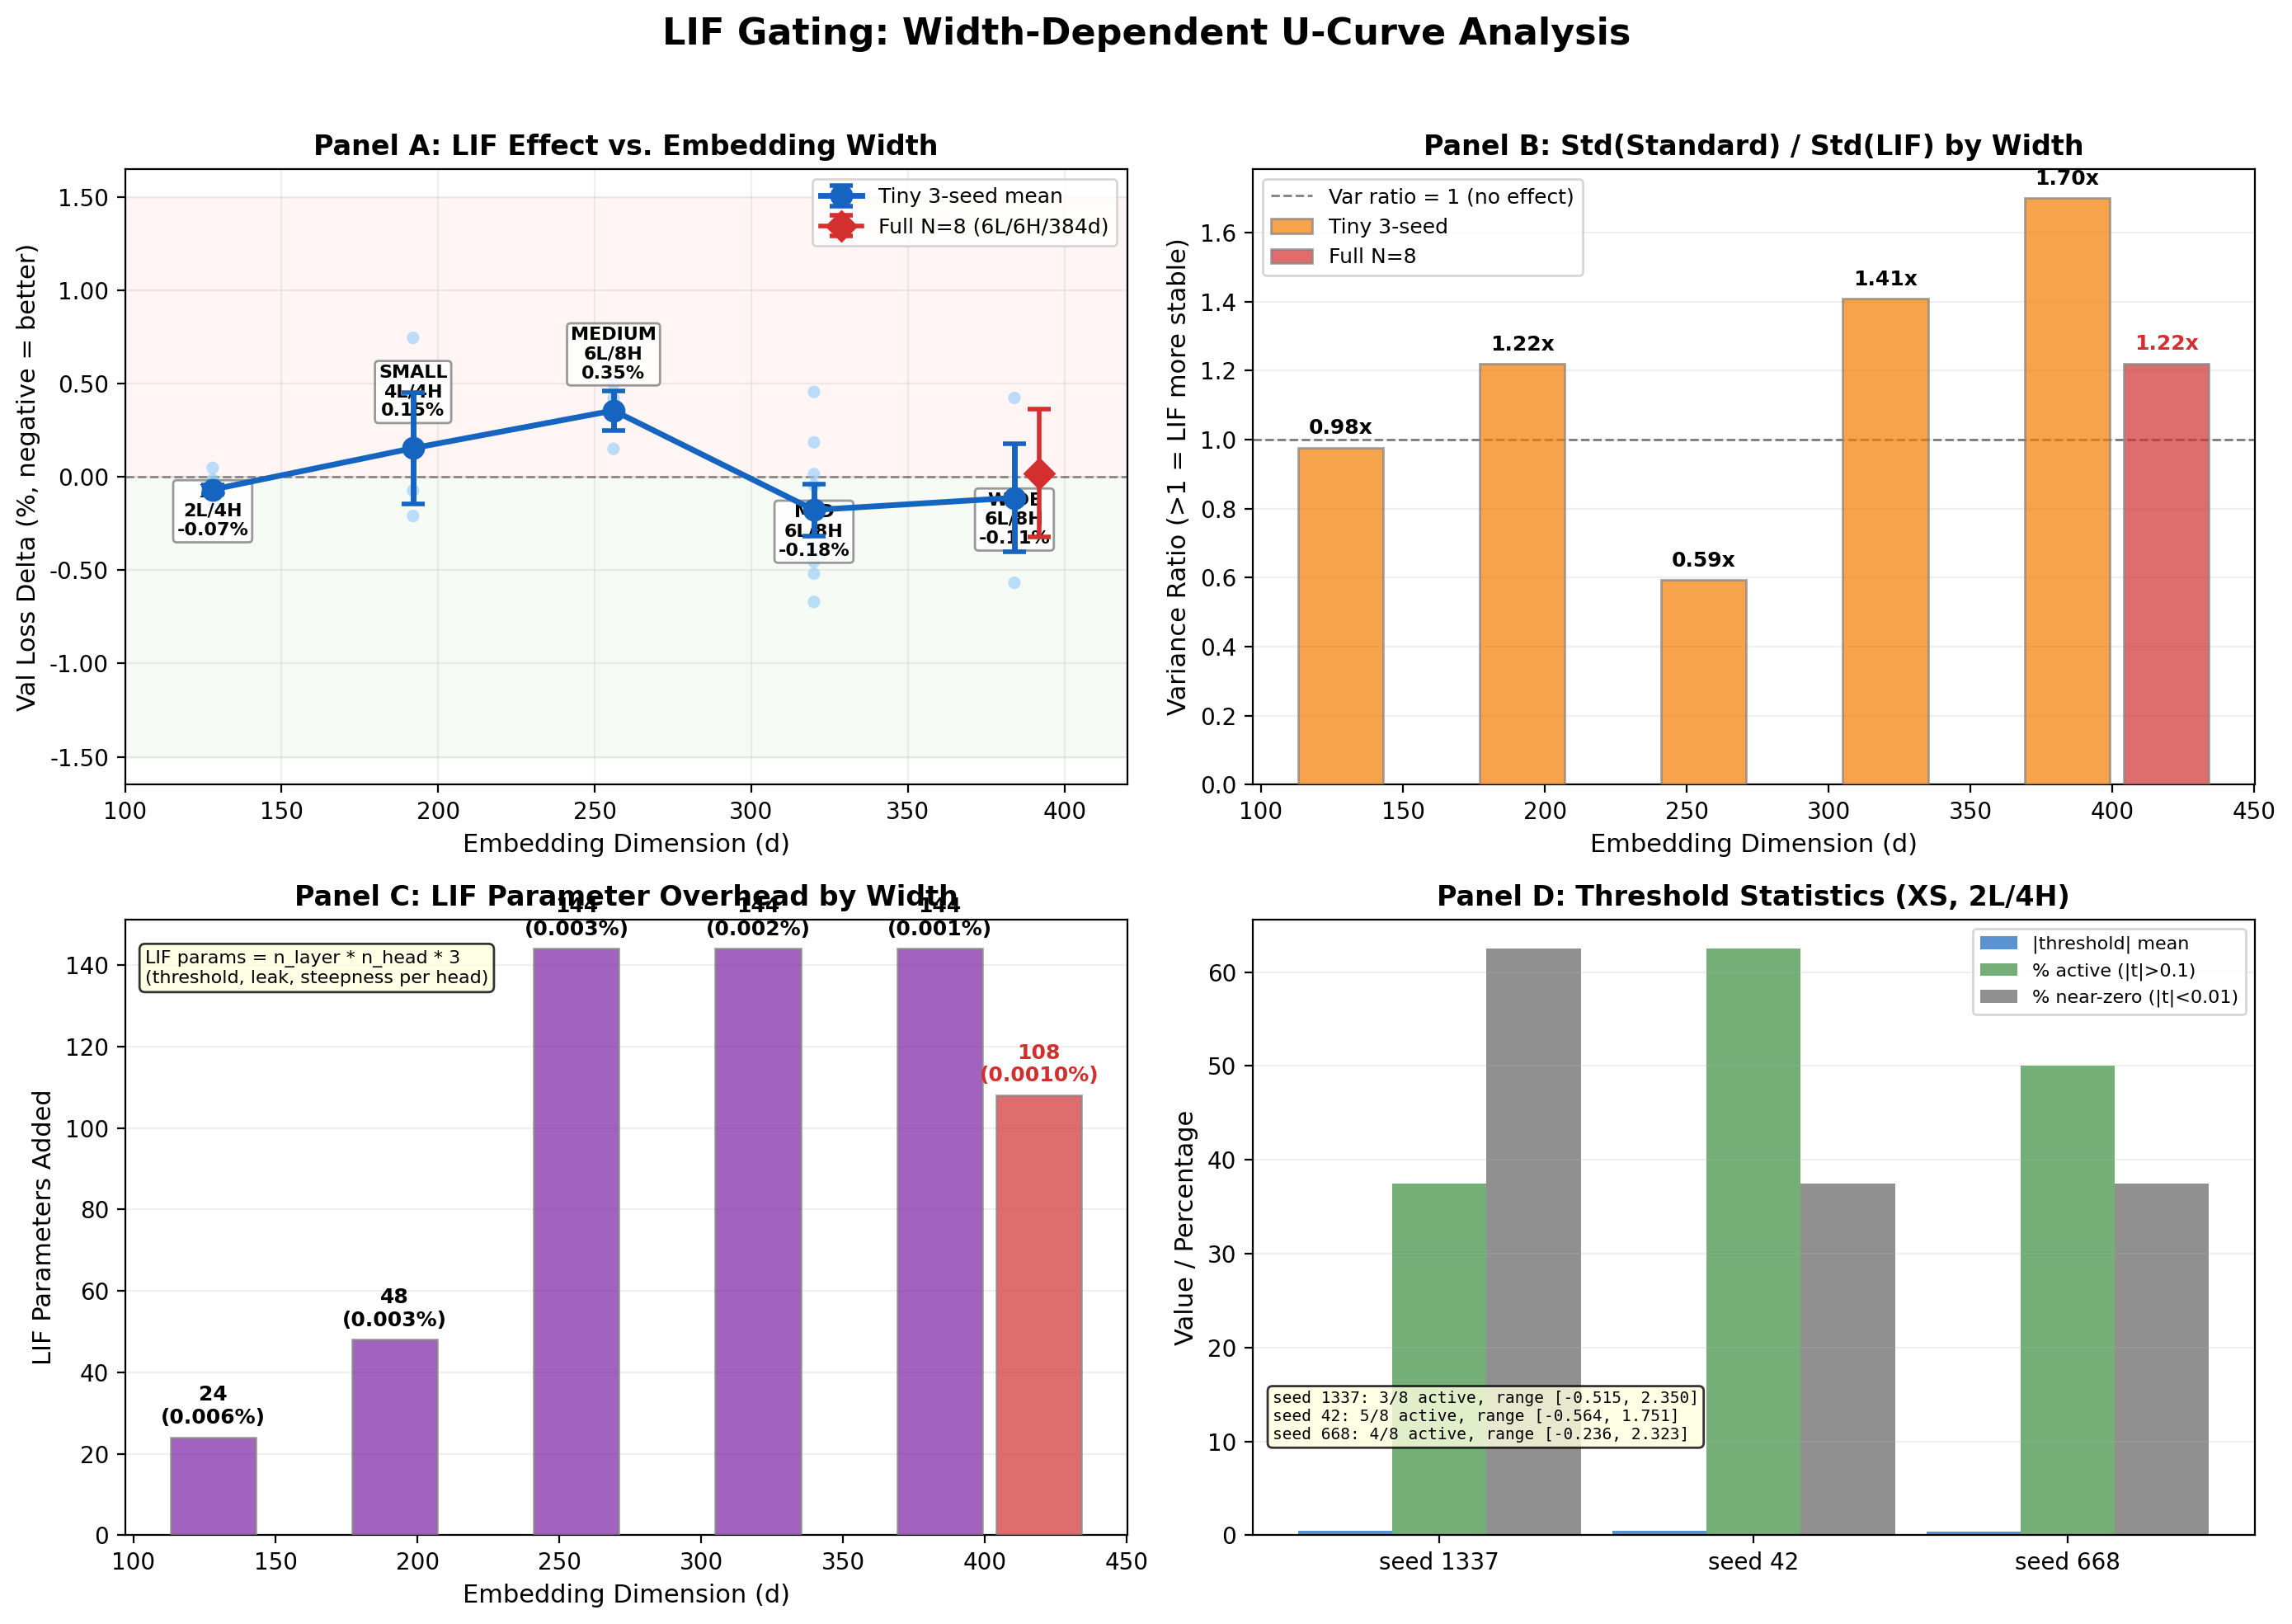
\includegraphics[width=\textwidth]{figures/u_curve_analysis.png}
\caption{\textbf{Width U-curve detailed analysis (4-panel).} Top-left: $\Delta$\% across 5 scales with 95\% CI, showing the U-shaped dependence with critical crossover between 256d--320d. Top-right: Cohen's $d$ effect size per scale. Bottom-left: statistical significance ($p$-values, dashed line at $\alpha = 0.05$). Bottom-right: per-seed $\Delta$ distributions. Four regimes emerge: \emph{constrained} (128d, LIF helps via selection pressure), \emph{neutral} (192d, no detectable effect at the crossover boundary), \emph{all-needed} (256d, LIF harms by removing useful dimensions), and \emph{redundant} (320d+, LIF helps as regularizer). See \S\ref{sec:width}.}
\label{fig:ucurve-detail}
\end{figure}

\begin{figure}[h]
\centering
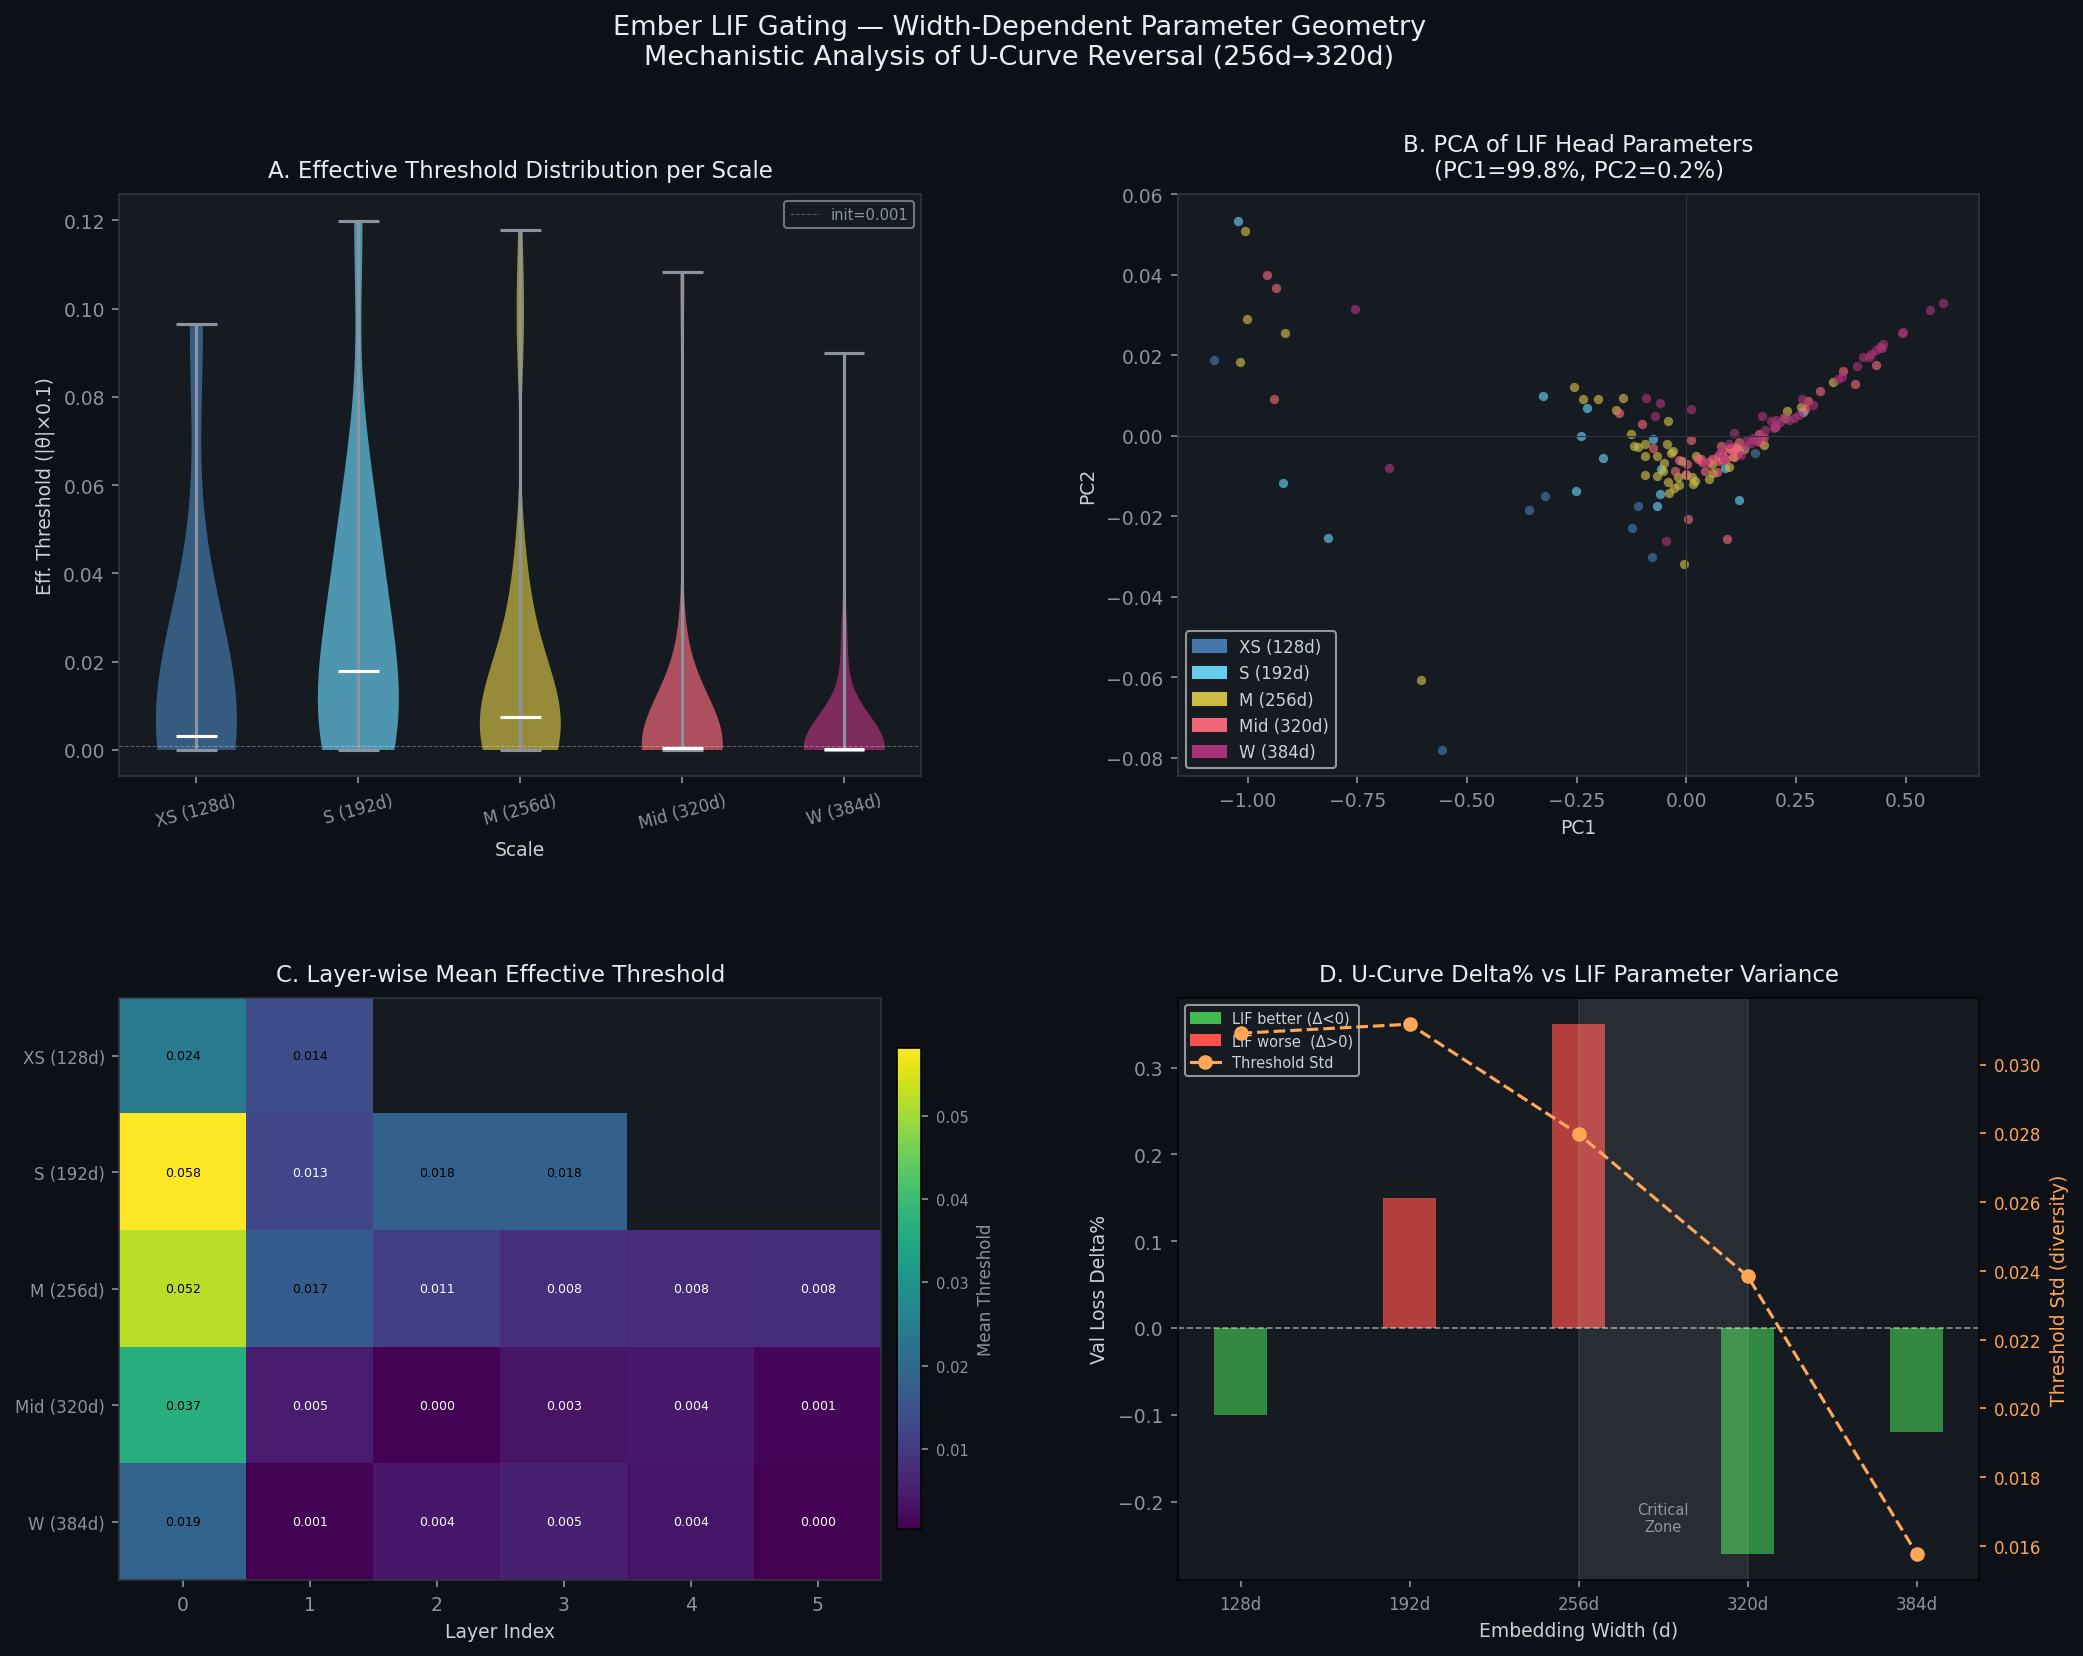
\includegraphics[width=\textwidth]{figures/lif_pca_width}
\caption{\textbf{LIF gating mechanistic analysis across scales (4-panel).}
(A)~Effective threshold distribution per scale (violin). Threshold standard
deviation decreases monotonically with width ($\sigma_\theta = 0.031$ at 128d
to $0.016$ at 384d), indicating reduced head-level diversity at wider scales.
(B)~PCA of per-head LIF parameters (threshold, leak, steepness) colored by scale.
Scales cluster along PC1, reflecting width-dependent parameter geometry.
(C)~Layer-wise mean effective threshold heatmap across scales.
(D)~U-curve $\Delta$\% (bars, green = LIF better) overlaid with threshold std
(orange line), revealing the mechanistic link: lower threshold diversity
correlates with reduced LIF efficacy in the medium regime (192--256d) and
recovery at wide scales (320d+) where representational redundancy allows
selective gating to re-emerge. Critical zone 256d--320d marked.
See \S\ref{sec:width}.}
\label{fig:lif-pca-width}
\end{figure}

\bibliography{references}

\end{document}
